\documentclass[a4paper]{panl}


\usepackage{cite}
\usepackage{wrapfig}
\usepackage{graphicx}
\usepackage{amssymb}
\usepackage{amsfonts}
\usepackage{amsmath}
\usepackage{longtable}
\usepackage{rotating}
\usepackage{lscape}
\usepackage{epsfig}
\usepackage{multirow}



\originalTeX
%\russianTeX
\begin{document}
% Journal sections (see http://pkp.jinr.ru/index.php/PEPAN_LETTERS/about/editorialPolicies#focusAndScope)
\issuearea{Physics of Elementary Particles and Atomic Nuclei. Theory}
% or in Russian
%\issuearea{ФИЗИКА ЭЛЕМЕНТАРНЫХ ЧАСТИЦ И АТОМНОГО ЯДРА. ТЕОРИЯ}

\title{Chemical composition analysis for X-ray transport container scans.  \\ Анализ химического состава при сканировании транспортных контейнеров гамма-излучением}
\maketitle
\authors{A. Zelenaya$^{~a}$, M. Zelenyi$^{~a,b,}$\footnote{E-mail: mihail.zelenyy@phystech.edu}, A.A.Turinge$^{~a}$,  V.G. Nedorezov$^{~a,}$\footnote{E-mail: vladimir@cpc.inr.ac.ru}}
\from{$^{a}$\,Institute of Nuclear Research of RAS}
\vspace{-3mm}
\from{$^{b}$\,Moscow Institute of Physical and Technology  (SU)}

\begin{abstract}
% Russian translation of the abstract
It is important for national security to control the movement of dangerous or strategically cargo such as explosives, radioactive materials, rare and precious metals. This control can be provided by scanning transport containers by gamma rays.
In this report the existing technique for scanning (dual energy method) is considered and the alternative method based on measuring the energy distribution of gamma rays is proposed. For estimation perspectives of the proposing method, the  corresponding simulation was conducted by using the GEANT4 toolkit. The example of the algorithm of reconstruction the chemical composition of the scanned object is also considered. In addition the experiment for estimation energy resolution of the detector based on a scintillation crystal BGO and SiPM was carried out.\\
\vspace{0.2cm}

Для обеспечения национальной безопасности важен контроль перемещения опасных или стратегически важных грузов, таких как взрывчатые вещества, радиоактивные материалы, редкие и драгоценные металлы. Проводить такой контроль можно сканирую содержимое   транспортных контейнеров гамма излучением. В данной работе рассмотрена существующая методика дуальных энергий и предложен альтернативный способ, основанный на измерении энергетического распределения гамма-квантов. Для оценки было проведено моделирование с помощью транспортного кода GEANT4.  Также выполнен эксперимент по измерению энергетического разрешения детектора на основе сцинтиллирующего кристалла BGO и кремневого фотоумножителя. 
\end{abstract}
\vspace*{6pt}

\noindent
PACS: 02.70.$-$c; 23.20.Nx; 32.90.$+$a

\label{sec:intro}
\section*{Introduction}
\newpage
\section*{Dual energy method}



\begin{figure}[t]
\begin{center}
    % Сделать подписи к отдельным картинкам
\includegraphics[width=60mm]{figures/Attenuation.pdf} 
\includegraphics[width=60mm]{figures/Bremsstrahlung.pdf}  
\vspace{-3mm}
\caption{a)Attenuation curve b) Bremsstrahlung spectrum by $10 MeV$ electron}
\end{center}
\labelf{fig01}
\vspace{-5mm}
\end{figure}

            $$
T(E_0, t, Z) = \frac{\int \limits_0^{E_0} S(E_0, E) \exp(-\mu(E,Z)\times t)~dE)}{\int \limits_0^{E_0} S(E_0, E)~dE}
$$
            $T$ -  transmittance, $S(E_0, E)$ - response function\\
$\mu(E,Z)$ - attenuation\\
$t$ -  optical thickness\\
$E_0$ -  up-limit energy of bremsstrahlung\\
$E$ - energy of gamma ray\\
$Z$ - charge of nuclei 
        \begin{itemize}
    \item We can't defined Z if optical thickness $t$ is unknown.
    \item But we can use two electron beams with different energy which give gamma rays with up-limit energy $E^{(1)}_0$ and $E^{(2)}_0$.
    \item Then we can get Z as a result of minimizing this function:
    $$
    F(z) = \frac{|t(E^{(1)}_0,z) - t(E^{(2)}_0,z)|}{t(E^{(1)}_0,z)} \to min
    $$
    \item This technique allows to determine scan object as a one from four possible groups: $Z_{eff} \sim 5$, $Z_{eff} \sim 13$, $Z_{eff} \sim 26$, $Z_{eff} \sim 82$.
\end{itemize}
Disadvantages of dual energy method
    \begin{itemize}
        \item It is too difficult to irradiate the target with beams with different energy.
        \item Low efficiency for target which contains elements with strongly different charges.
    \end{itemize}
Our method
    \begin{itemize}
        \item Use only one electron beam with energy $E = 10 MeV$.
        \item Measure not only the space distribution, but also the energy of gamma rays.
    \end{itemize}

\section*{Simulation}
\begin{figure}[t]
    \begin{center}
        % Сделать подписи к отдельным картинкам
        \includegraphics[width=120mm]{figures/yed_schema_1.pdf}  
        \vspace{-3mm}
        \caption{a) }
    \end{center}
    \labelf{fig01}
    \vspace{-5mm}
\end{figure}
\begin{figure}[t]
    \begin{center}
        % Сделать подписи к отдельным картинкам
        % Переделать картинку от Туринге
        \includegraphics[width=60mm]{figures/Sword.pdf} 
        \includegraphics[width=60mm]{figures/Sword.pdf}  
        \vspace{-3mm}
        \caption{a) b)}
    \end{center}
    \labelf{fig01}
    \vspace{-5mm}
\end{figure}
\begin{figure}[t]
    \begin{center}
        % Сделать подписи к отдельным картинкам
        % Переделать картинку от Туринге
        \includegraphics[width=60mm]{figures/Difference.pdf} 
        \includegraphics[width=60mm]{figures/Difference.pdf}  
        \vspace{-3mm}
        \caption{a) b)}
    \end{center}
    \labelf{fig01}
    \vspace{-5mm}
\end{figure}


\section*{Thickness reconstruction}

\begin{figure}[t]
    \begin{center}
        % Сделать подписи к отдельным картинкам
        \includegraphics[width=120mm]{figures/yed_schema_2.pdf}  
        \vspace{-3mm}
        \caption{a) }
    \end{center}
    \labelf{fig01}
    \vspace{-5mm}
\end{figure}
                Attenuation of gamma ray flux is defined as:
$$
\frac{N(E)}{N_0(E)} = \exp(-\sum_i \Sigma^{mean}_i(E)x_i)
$$
where $x_i$ --- thickness of the $i$-layer, $\Sigma^{mean}_i$ --- mean cross-section for group of materials, $N,~N_0$ --- the number of gamma.
\begin{itemize}
    \item Disregard secondary scattering.
    \item Disregard the annihilation line.
\end{itemize}

                    \begin{itemize}
    \item Full thickness is known.
    \item Find thickness using least squares:                  
    
\end{itemize}
$$
\sum_E(\ln \frac{N(E)}{N_0(E)} + \sum_i \Sigma^{mean}_i(E)x_i))^2 \to min
$$

\begin{figure}[t]
    \begin{center}
        % Сделать подписи к отдельным картинкам
        \includegraphics[width=60mm]{figures/reconstruction.pdf} 
        \includegraphics[width=60mm]{figures/relError.pdf}  
        \vspace{-3mm}
        \caption{a) b)Distribution of reconstruction errors for various numerical experiments}
    \end{center}
    \labelf{fig01}
    \vspace{-5mm}
\end{figure}

\section*{Experiment}
The experiment was conducted by Dr. Guber and Dr. Ivashkin.
The sum of signals from 2 photodiode\\
Noise threshold: 100 KeV\\
\begin{center}
    \begin{tabular}[c]{|c|c|c|}
    \hline 
    Source & Energy, MeV & Sigma/Mean \\
    \hline 
    $^{22}Na$&0.511 & 14.7\%  \\ 
    \hline 
    $^{137}Cs$&0.662 & 19\%\\ 
    \hline 
    $^{22}Na$& 1.275 & 13\% \\
    \hline 
\end{tabular} 
\end{center}

\begin{figure}[t]
    \begin{center}
        % Сделать подписи к отдельным картинкам
        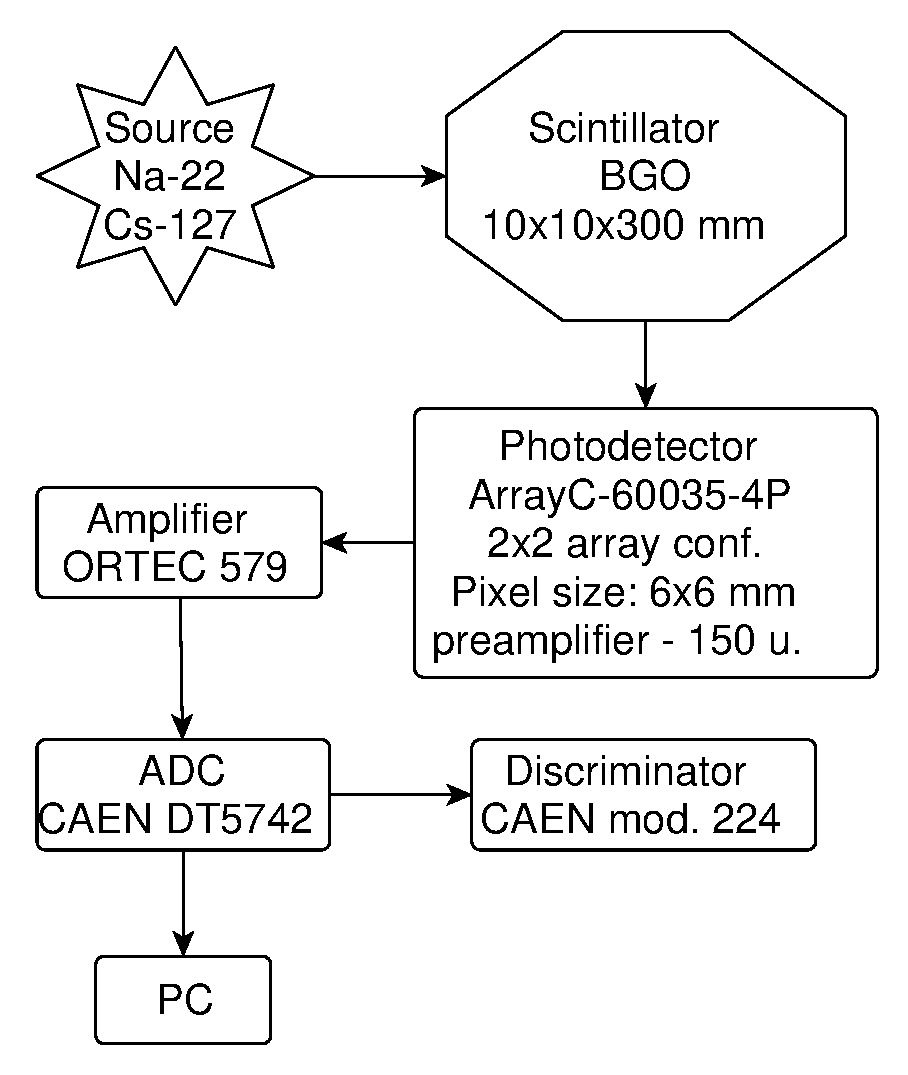
\includegraphics[width=80mm]{figures/yed.pdf}  
        \vspace{-3mm}
        \caption{a) }
    \end{center}
    \labelf{fig01}
    \vspace{-5mm}
\end{figure}
\section*{Conclusion}
% Выводы сделать более твердыми и акцентирванными
Results:   
    \begin{enumerate}
        \item The measurement of the gamma ray spectrum allows to identify cargo belonging to the group of materials with certain $Z_{eff}$.
        \item Also it allows to define the thickness of layers from different elements with the accuracy about 25\%.
        \item The energy resolution of the detector based on a BGO scintillator was studied.  For the photodetector with full array of pixels the energy resolution is expected about 10\%.
    \end{enumerate}
Plans and perspectives
    With financial support can be developed:
    \begin{enumerate}
        \item The program which checks cargo of a transport container  for compliance cargo manifest
        \item The algorithm for the 3D gamma-tomography.
    \end{enumerate}

This work is supported by the Ministry of Education and Science of the Russian Federation under the contract No. 3.3008.2017/PP.


%============================= Fig. 1 ================================
%\begin{figure}[t]
%\begin{center}
%\includegraphics[width=127mm]{fig_1.eps} 
%%\includegraphics[width=127mm]{fig_1.eps} 
%\vspace{-3mm}
%\caption{Figure caption}
%\end{center}
%\labelf{fig01}
%\vspace{-5mm}
%\end{figure}
%============================= Fig. 1 ================================


%\nocite{*}
\bibliographystyle{pepan}
\bibliography{pepan_biblio}

\end{document}
